\hypertarget{protocol_t_p_axis_style-p}{
\section{$<$ TPAxisStyle $>$ Protocol Reference}
\label{protocol_t_p_axis_style-p}\index{TPAxisStyle-p@{TPAxisStyle-p}}
}
{\tt \#import $<$TPParameterProtocols.h$>$}

Inheritance diagram for $<$ TPAxisStyle $>$::\begin{figure}[H]
\begin{center}
\leavevmode
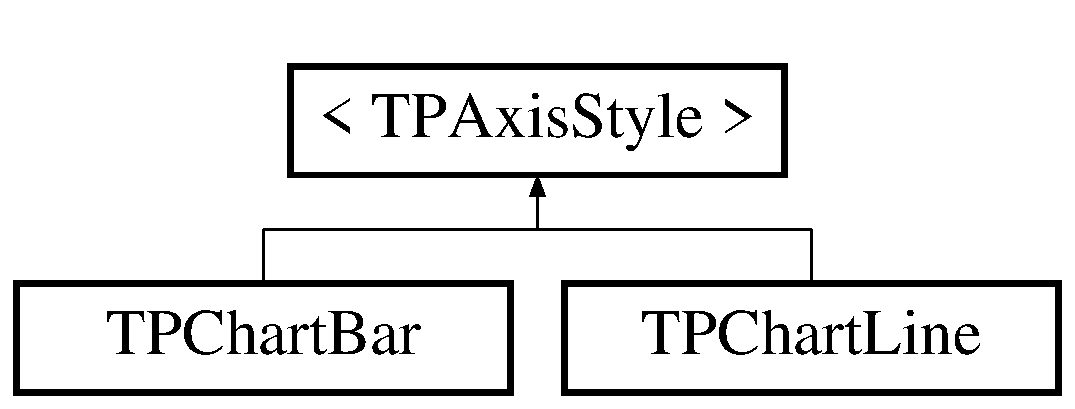
\includegraphics[height=2cm]{protocol_t_p_axis_style-p}
\end{center}
\end{figure}
\subsection*{Public Member Functions}
\begin{CompactItemize}
\item 
(void) - \hyperlink{protocol_t_p_axis_style-p_2e524aea66679aa46e6456b64c9327ec}{setAxisStyle:}
\end{CompactItemize}


\subsection{Detailed Description}
Protocol for charts who can have axis 

\subsection{Member Function Documentation}
\hypertarget{protocol_t_p_axis_style-p_2e524aea66679aa46e6456b64c9327ec}{
\index{TPAxisStyle-p@{TPAxisStyle-p}!setAxisStyle:@{setAxisStyle:}}
\index{setAxisStyle:@{setAxisStyle:}!TPAxisStyle-p@{TPAxisStyle-p}}
\subsubsection[{setAxisStyle:}]{\setlength{\rightskip}{0pt plus 5cm}- (void) setAxisStyle: ({\bf TPParameterAxisStyle} $\ast$) {\em style}}}
\label{protocol_t_p_axis_style-p_2e524aea66679aa46e6456b64c9327ec}


sets the axis style for the receiving chart \begin{Desc}
\item[Parameters:]
\begin{description}
\item[{\em style}]axis style \end{description}
\end{Desc}


The documentation for this protocol was generated from the following file:\begin{CompactItemize}
\item 
TPParameterProtocols.h\end{CompactItemize}
